% /chapters/2-descriptive-combinatorics/01-background.tex

\section{Background}\label{sec:descr_combi_background}

Throughout this entire chapter, $G$ denotes an analytic graph on a Polish space $V(G)=X$.
That is, $X$ is a separable completely metrizable topological space, and $G$ is a symmetric and irreflexive relation on $X$ which, as a subspace of $X\times X$, is the continuous image of a Polish space.%
\footnote{In contrast with graph-theoretical literature, in this context it is customary to use the variable $G$ as the set of edges. The difference is inessential.}

We employ the symbol $H\to_cG$ (respectively, $H\to_BG$) to abbreviate the fact that there is a continuous (respectively Borel) homomorphism from the analytic graph $H$ to the analytic graph $G$.

\subsection{The Borel chromatic number}\label{subsec:borel-chromatic-numbers}

Recall the \emph{$\mathbb{G}_0$ dichotomy} from Chapter~\ref{ch:introduction}: there exists a Borel graph~$\mathbb{G}_0$ such that
\begin{align}\label{eq:G0-dichotomy}
    \chi_B(G) > \aleph_0\quad
    \Longleftrightarrow\quad
    \mathbb{G}_0 \to_B G.
\end{align}

This dichotomy breaks down when one moves from uncountable to merely infinite Borel chromatic number.
In \cite{Todorcevic_2021_ComplexProbBorel}, Todor{\v{c}}evi{\'c} and Vidny{\'{a}}nszky proved that the set of Borel graphs with infinite Borel chromatic number is $\mathbf\Sigma^1_2$-complete; their reduction in fact gives the same conclusion for closed subgraphs of the shift graph at the threshold $\chi_B\geq 4$.
In particular, no countable family of Borel graphs can serve as a basis for this class.
Moreover, their argument rules out the existence of a simple $\mathbb{G}_0$-type dichotomy substituting $\aleph_0$ in \eqref{eq:G0-dichotomy} for any $k\geq3$.
Interestingly, when substituting the value $2$, there again is a single Borel graph that makes a dichotomy like \eqref{eq:G0-dichotomy} hold.
This is known as the $\mathbb{L}_0$~dichotomy, a result first established in \cite{L0paper} and proved concisely in Section~\ref{sec:concise_L0}.

A common situation is having an analytic set and the desire to apply to it a statement that holds for Borel sets instead.
One way to circumvent this problem is by using Borel separation to ``inflate'' the analytic set into a Borel set with the same property.
This technique is crucial, for instance, for the proof of the $\mathbb{G}_0$ dichotomy found in \cite{Bernshteyn2024}.
Concretely, since the dichotomy is a statement about independent sets of vertices, the proof makes use of the following fact.

\begin{proposition}\label{prop:indep-analyitc-borel}
    In the graph $G$, any analytic independent set of vertices is contained in a Borel independent set.\footnote{In the case that $X$ is finite, this Proposition becomes trivial; see Remark~\ref{rmk:finite-Borel}.}
\end{proposition}

We present two proofs of this fact, original to this exposition, for several reasons.
First, because \cite{Bernshteyn2024} omits it;\footnote{The fact is indeed left as an exercise to the reader in \cite{Bernshteyn2024}.} it is an illustrative example of how different notions of separation get used in an argument; and it motivates the introduction of a more powerful technique required in Section~\ref{sec:concise_L0}.
Specifically, Claim~\ref{claim:separation_odd-walks} states an analogous result for odd-walks, instead of merely independent sets.
The added complexity is that odd-walks can have different lengths, and so proving the aforementioned claim is not as straightforward without invoking Lemma~\ref{lemma:first-reflection}.

\begin{proof}
    Suppose that $I \subseteq V(G)$ is an analytic independent set.
    We view the edge relation of $G$ as a subset of $V(G)\times V(G)$, which is analytic by assumption.

    First, consider the set $$A_0 := \{x_0\in V(G):\exists x_1\in I\ (x_0x_1\in G)\},$$
    which consists of all vertices with at least one neighbour in $I$.
    To see that $A_0$ is analytic, write it as the projection onto the first coordinate of the set $$(V(G)\times I)\cap G \;=\; \{(x_0,x_1): x_1\in I \text{ and } x_0x_1\in G\}.$$
    This is the intersection of the analytic set $V(G)\times I$ with the analytic set $G$, hence analytic.
    Since $I$ is independent, $I\cap A_0=\emptyset$.
    As $I$ and $A_0$ are disjoint analytic sets, the Lusin Separation Theorem \cite[Theorem~14.7]{Kechris_1995_DescriptiveSetTheory} yields a Borel set $B_0\subseteq V(G)$ with $$I\subseteq B_0 \quad\text{and}\quad B_0\cap A_0=\emptyset.$$
    The second condition means that no vertex of $B_0$ has any neighbour in $I$.

    Next, let $$A_1 := \{x_1\in V(G):\exists x_0\in B_0\ (x_0x_1\in G)\}$$
    be the set of all vertices with at least one neighbour in $B_0$.
    Analogously to before, $A_1$ is the projection onto the second coordinate of
    $$(B_0\times V(G))\cap G \;=\; \{(x_0,x_1): x_0\in B_0 \text{ and } x_0x_1\in G\},$$
    which is the intersection of the Borel set $B_0\times V(G)$ with the analytic set $G$, and is therefore analytic.
    We claim that $I\cap A_1=\emptyset$.
    Indeed, if some $x_1\in I$ had a neighbour $x_0\in B_0$, then $x_0$ would be a vertex of $B_0$ with a neighbour $x_1\in I$, that is $x_0\in A_0$, contradicting $B_0\cap A_0=\emptyset$.
    So again we have two disjoint analytic sets, and separation yields a Borel set $B_1\subseteq V(G)$ with $$I\subseteq B_1 \quad\text{and}\quad B_1\cap A_1=\emptyset.$$
    The second condition means that no vertex of $B_1$ has any neighbour in $B_0$.

    Set $B:=B_0\cap B_1$, which is Borel and contains $I$.
    It remains to check that $B$ is independent.
    Suppose for contradiction that $x_0,x_1\in B$ with $x_0x_1\in G$.
    Then $x_0\in B_0$, so $x_1$ is a vertex with a neighbour in $B_0$, giving $x_1\in A_1$.
    But $x_1\in B_1$ and $B_1\cap A_1=\emptyset$, a contradiction.
\end{proof}

\begin{figure}[ht]
    \centering
    % figures/Borel-separation.tex

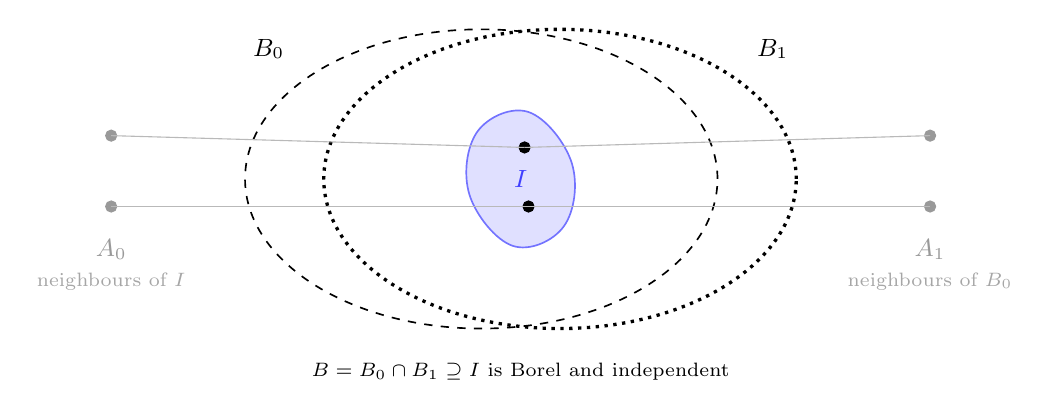
\begin{tikzpicture}[font=\small]

  % B0 -- dashed ellipse, offset left
  \draw[dashed, semithick] (-0.5, 0) ellipse (3.0 and 1.9);
  \node at (-3.2, 1.65) {$B_0$};

  % B1 -- dotted ellipse, offset right
  \draw[dotted, semithick, line width=1.2pt] (0.5, 0) ellipse (3.0 and 1.9);
  \node at (3.2, 1.65) {$B_1$};

  % I -- organic blob sitting in the intersection
  \filldraw[fill=blue!12, draw=blue!55, semithick]
    plot[smooth cycle, tension=0.65] coordinates {
      ( 0.10,  0.85) ( 0.65,  0.20) ( 0.55, -0.60)
      (-0.10, -0.85) (-0.65, -0.20) (-0.55,  0.60)
    };
  \node[blue!75] at (0, 0) {$I$};

  % Two vertices inside I
  \filldraw (0.05,  0.40) circle (2pt) coordinate (v1);
  \filldraw (0.10, -0.35) circle (2pt) coordinate (v2);

  % A0 -- neighbours of I, outside B0  (B0 reaches to x = -3.5)
  \filldraw[gray!80] (-5.2,  0.55) circle (2pt) coordinate (a01);
  \filldraw[gray!80] (-5.2, -0.35) circle (2pt) coordinate (a02);
  \node[gray!80]             at (-5.2, -0.90) {$A_0$};
  \node[gray!70, font=\scriptsize] at (-5.2, -1.30) {neighbours of $I$};

  % A1 -- neighbours of B0, outside B1  (B1 reaches to x = +3.5)
  \filldraw[gray!80] (5.2,  0.55) circle (2pt) coordinate (a11);
  \filldraw[gray!80] (5.2, -0.35) circle (2pt) coordinate (a12);
  \node[gray!80]             at (5.2, -0.90) {$A_1$};
  \node[gray!70, font=\scriptsize] at (5.2, -1.30) {neighbours of $B_0$};

  % Edges from I to A0 (cross the B0 boundary)
  \draw[gray!55, thin] (v1) -- (a01);
  \draw[gray!55, thin] (v2) -- (a02);

  % Edges from I (subset of B0) to A1 (cross the B1 boundary)
  \draw[gray!55, thin] (v1) -- (a11);
  \draw[gray!55, thin] (v2) -- (a12);

  % Caption
  \node[font=\scriptsize] at (0, -2.45)
    {$B = B_0 \cap B_1 \supseteq I$ is Borel and independent};

\end{tikzpicture}
    \caption{An illustration of Borel Separation in vertex sets.}
    \label{fig:Borel_separation}
\end{figure}

The following notion, taken from \cite[Theorem~35.10, p.~285]{Kechris_1995_DescriptiveSetTheory}, is a well-known fact about analytic sets.

\begin{definition}\label{def:pi11-on-sigma11}
    Let $X$ be a Polish space and let $\Phi\subseteq\mathcal P(X)$.
    We say $\Phi$ is \emph{$\Pi^1_1$ on $\Sigma^1_1$} if for any Polish $Y$ and any $\Sigma^1_1$ set $A\subseteq Y\times X$, the set $A_\Phi:=\{y\in Y:A_y\in\Phi\}$, where $A_y:=\{x\in X:(y,x)\in A\}$, is $\Pi^1_1$.
\end{definition}

\begin{lemma}[First Reflection Theorem]\label{lemma:first-reflection}
    If $\Phi$ is as in the preceding definition, then for any $\Sigma^1_1$ set $A\in\Phi$, there is a Borel set $B\subseteq X$ such that $A\subseteq B$ and $B\in\Phi$.
\end{lemma}

For example, the property of being an independent set of vertices is, as expected, $\Pi^1_1$ on $\Sigma^1_1$.
Indeed, let $\Phi$ denote the collection of all independent subsets of $V(G)$, let $Y$ be a Polish space, and let $A\subseteq Y\times V(G)$ be $\Sigma^1_1$.
We must show that $A_\Phi=\{y\in Y: A_y\in\Phi\}$ is $\Pi^1_1$.
Observe that its complement consists precisely of those $y\in Y$ for which $A_y$ contains an edge:
$$Y\setminus A_\Phi = \{y\in Y:\exists x_0,x_1\in V(G)\ (x_0x_1\in G\wedge (y,x_0)\in A\wedge (y,x_1)\in A)\}.$$
The set $\{(y,x_0,x_1): (y,x_0)\in A\wedge (y,x_1)\in A\}$ is $\Sigma^1_1$, being the preimage of $A\times A$ under the continuous map $(y,x_0,x_1)\mapsto ((y,x_0),(y,x_1))$; intersecting with the $\Sigma^1_1$ set $\{(y,x_0,x_1): x_0x_1\in G\}$ keeps it $\Sigma^1_1$.
Projecting onto $Y$ therefore yields a $\Sigma^1_1$ set, so $A_\Phi$ is $\Pi^1_1$, as required.

Consequently, Proposition~\ref{prop:indep-analyitc-borel} is an immediate corollary of Lemma~\ref{lemma:first-reflection}: given an analytic independent set $I\in\Phi$, the First Reflection Theorem directly produces a Borel set $B\supseteq I$ with $B\in\Phi$.
Note that this second proof, unlike the elementary one given above, generalises readily: one only needs to verify the $\Pi^1_1$ on $\Sigma^1_1$ property for the relevant family $\Phi$, which, for more complex combinatorial properties, is typically a non-trivial step.

\subsection{The Borel dichromatic number}

All of the foregoing has been about undirected graphs; we now turn to the directed setting, where the basis landscape is richer and only partially understood.
The \emph{dichromatic number} of a directed graph was introduced by Neumann-Lara~\cite{NeumannLara1982} as a natural directed analogue of the chromatic number.
In a \emph{directed graph}, instead of having a set of edges as unordered pairs of vertices, we consider ordered pairs of vertices, called \emph{arcs}.
A \emph{dicolouring} of a directed graph~$D$ is a map $c\colon V(D)\to k$ such that every colour class induces a subgraph without any directed cycles; the \emph{dichromatic number} $\vec\chi(D)$ is the least such~$k$.
Equivalently, $\vec\chi(D)$ is the minimum number of vertex sets inducing acyclic subgraphs.

The following table summarizes the basis landscape, contrasting the undirected and directed cases at different thresholds.

\medskip
\begin{center}
\begin{tabular}{lll}
	\hline
	\textbf{Class} & \textbf{Existence of a countable basis} & \textbf{Reference} \\
	\hline
	$\chi_B(G) > \aleph_0$ & Yes (size 1: $\mathbb{G}_0$) & \cite{kechris1999borel} \\
	$\chi_B(G) > 2$ & Yes (size 1: $\mathbb{L}_0$) & \cite{L0paper}, Section~\ref{sec:concise_L0} \\
	$\chi_B(G) > k$, $k\geq 3$ & No ($\mathbf\Pi^1_2$-complete) & \cite{Todorcevic_2021_ComplexProbBorel} \\
	\hline
	$\vec\chi_B(D) > \aleph_0$ & No (size $\mathfrak{c}$ basis exists) & \cite{RaghavanXiao2024} \\
	$\vec\chi_B(D) > k$, $k\geq 2$ & No ($\mathbf\Pi^1_2$-complete) & Prop.~\ref{prop:main}, Rmk.~\ref{rmk:dichrom-recovers-chrom} \\
	\hline
\end{tabular}
\end{center}

The notion of dichromatic number has attracted considerable attention in finite combinatorics.
Neumann-Lara~\cite{NeumannLara1982} established several foundational results, including analogues of classical lower bounds for the chromatic number.
Bokal, Fijav{\v{z}}, Juvan, Kayll, and Mohar~\cite{Bokal_2004_CircularChrom} later introduced the circular dichromatic number of a directed graph and proved that the decision problem of whether a directed graph $D$ satisfies $\vec\chi(D)\leq 2$ or not is NP-complete; this is in contrast with the usual chromatic number for (undirected) graphs, where one gets NP-completeness only after posing the question for three colours or more.

Very recently, Raghavan and Xiao~\cite{RaghavanXiao2024} established a dichotomy for the Borel dichromatic number that generalizes the $\mathbb{G}_0$ dichotomy to directed graphs: they showed that a continuum-size family of directed graphs characterizes when a Borel directed graph has uncountable Borel dichromatic number.
This continuum-size basis consists of pairwise Borel-incomparable directed graphs, but it is unknown whether any smaller basis exists; in particular, the question of whether a \emph{countable} basis suffices is open.

The Borel dichromatic number can recover the Borel chromatic number in the following sense.

\begin{remark}\label{rmk:dichrom-recovers-chrom}
	Given an undirected graph $G$, let $\vec{G}$ denote the directed graph obtained by replacing each edge $\{u,v\}$ with two opposing arcs $(u,v)$ and $(v,u)$.
	Then $\vec\chi_B(\vec{G}) = \chi_B(G)$.
	Indeed, a subset of vertices is acyclic in $\vec{G}$ if and only if it is independent in~$G$: any directed cycle in $\vec{G}$ would in particular contain an arc $(u,v)$ with $uv\in G$, so a set containing both $u$ and $v$ is neither acyclic in $\vec{G}$ nor independent in~$G$; conversely, an independent set in~$G$ induces a directed graph in~$\vec{G}$ with no arcs at all, hence trivially acyclic.
	Moreover, the map $\mathrm{code}(G)\mapsto\mathrm{code}(\vec{G})$ is $\Delta^1_1$, since it is built from the edge set using products and unions (Lemma~\ref{lemma:toolkit}(1),(3)).
	It follows that the $\mathbf\Sigma^1_2$-completeness of Borel $k$-colouring of undirected graphs~\cite{Todorcevic_2021_ComplexProbBorel} implies the $\mathbf\Sigma^1_2$-completeness of Borel $k$-dicolouring of directed graphs, for every $k\geq 3$.
	The case $k=2$ is not covered by this reduction (since deciding 2-colourability of undirected graphs is trivial algorithmically, hence not $\Sigma^1_2$-complete in the relevant sense), and is precisely the content of Proposition~\ref{prop:main}.
\end{remark}

It is natural to ask whether the Todor{\v{c}}evi{\'c}--Vidny{\'{a}}nszky phenomenon also occurs in the directed setting at the remaining finite threshold, or if there is a directed analogue for the $\mathbb{L}_0$ dichotomy:

\begin{quote}
\emph{Is there a countable basis for the class of Borel directed graphs with Borel dichromatic number at least~$3$?}
\end{quote}

Section~\ref{sec:dichromatic} gives a negative answer, thereby completing the picture for all finite thresholds of both the Borel chromatic and dichromatic numbers.